% Created by tikzDevice version 0.11 on 2018-05-19 10:35:13
% !TEX encoding = UTF-8 Unicode
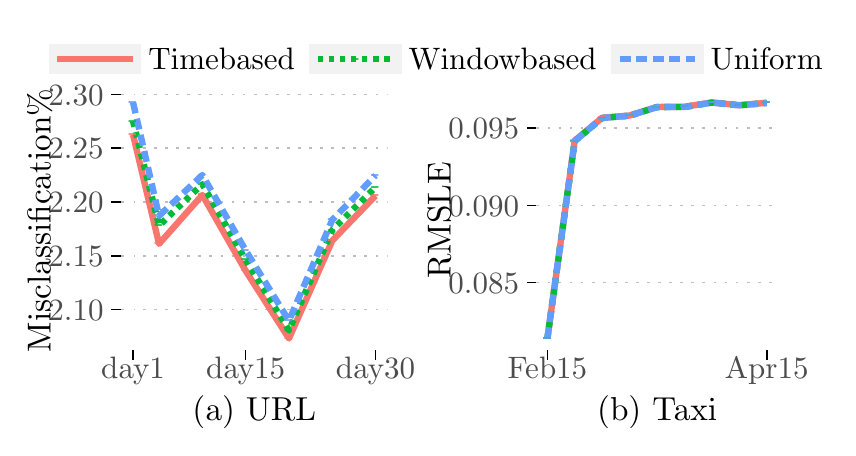
\begin{tikzpicture}[x=1pt,y=1pt]
\definecolor{fillColor}{RGB}{255,255,255}
\path[use as bounding box,fill=fillColor,fill opacity=0.00] (0,0) rectangle (289.08,144.54);
\begin{scope}
\path[clip] (  0.00,  0.00) rectangle (289.08,144.54);
\definecolor{fillColor}{RGB}{255,255,255}

\path[fill=fillColor] ( -2.74,121.78) rectangle (291.82,144.54);
\end{scope}
\begin{scope}
\path[clip] (  0.00,  0.00) rectangle (289.08,144.54);
\definecolor{drawColor}{RGB}{0,0,0}

\node[text=drawColor,anchor=base west,inner sep=0pt, outer sep=0pt, scale=  0.00] at (  2.95,133.16) {Sampling};
\end{scope}
\begin{scope}
\path[clip] (  0.00,  0.00) rectangle (289.08,144.54);
\definecolor{drawColor}{RGB}{255,255,255}
\definecolor{fillColor}{gray}{0.95}

\path[draw=drawColor,line width= 0.6pt,line join=round,line cap=round,fill=fillColor] (  7.28,127.47) rectangle ( 41.43,138.85);
\end{scope}
\begin{scope}
\path[clip] (  0.00,  0.00) rectangle (289.08,144.54);
\definecolor{drawColor}{RGB}{248,118,109}

\path[draw=drawColor,line width= 2.3pt,line join=round] ( 10.70,133.16) -- ( 38.01,133.16);
\end{scope}
\begin{scope}
\path[clip] (  0.00,  0.00) rectangle (289.08,144.54);
\definecolor{drawColor}{RGB}{248,118,109}

\node[text=drawColor,anchor=base,inner sep=0pt, outer sep=0pt, scale=  1.00] at ( 24.36,131.00) {-};
\end{scope}
\begin{scope}
\path[clip] (  0.00,  0.00) rectangle (289.08,144.54);
\definecolor{drawColor}{RGB}{255,255,255}
\definecolor{fillColor}{gray}{0.95}

\path[draw=drawColor,line width= 0.6pt,line join=round,line cap=round,fill=fillColor] (101.38,127.47) rectangle (135.52,138.85);
\end{scope}
\begin{scope}
\path[clip] (  0.00,  0.00) rectangle (289.08,144.54);
\definecolor{drawColor}{RGB}{0,186,56}

\path[draw=drawColor,line width= 2.3pt,dash pattern=on 2pt off 2pt ,line join=round] (104.79,133.16) -- (132.10,133.16);
\end{scope}
\begin{scope}
\path[clip] (  0.00,  0.00) rectangle (289.08,144.54);
\definecolor{drawColor}{RGB}{0,186,56}

\node[text=drawColor,anchor=base,inner sep=0pt, outer sep=0pt, scale=  1.00] at (118.45,131.00) {-};
\end{scope}
\begin{scope}
\path[clip] (  0.00,  0.00) rectangle (289.08,144.54);
\definecolor{drawColor}{RGB}{255,255,255}
\definecolor{fillColor}{gray}{0.95}

\path[draw=drawColor,line width= 0.6pt,line join=round,line cap=round,fill=fillColor] (210.47,127.47) rectangle (244.61,138.85);
\end{scope}
\begin{scope}
\path[clip] (  0.00,  0.00) rectangle (289.08,144.54);
\definecolor{drawColor}{RGB}{97,156,255}

\path[draw=drawColor,line width= 2.3pt,dash pattern=on 4pt off 2pt ,line join=round] (213.88,133.16) -- (241.20,133.16);
\end{scope}
\begin{scope}
\path[clip] (  0.00,  0.00) rectangle (289.08,144.54);
\definecolor{drawColor}{RGB}{97,156,255}

\node[text=drawColor,anchor=base,inner sep=0pt, outer sep=0pt, scale=  1.00] at (227.54,131.00) {-};
\end{scope}
\begin{scope}
\path[clip] (  0.00,  0.00) rectangle (289.08,144.54);
\definecolor{drawColor}{RGB}{0,0,0}

\node[text=drawColor,anchor=base west,inner sep=0pt, outer sep=0pt, scale=  1.12] at ( 43.60,129.30) {Timebased};
\end{scope}
\begin{scope}
\path[clip] (  0.00,  0.00) rectangle (289.08,144.54);
\definecolor{drawColor}{RGB}{0,0,0}

\node[text=drawColor,anchor=base west,inner sep=0pt, outer sep=0pt, scale=  1.12] at (137.69,129.30) {Windowbased};
\end{scope}
\begin{scope}
\path[clip] (  0.00,  0.00) rectangle (289.08,144.54);
\definecolor{drawColor}{RGB}{0,0,0}

\node[text=drawColor,anchor=base west,inner sep=0pt, outer sep=0pt, scale=  1.12] at (246.78,129.30) {Uniform};
\end{scope}
\begin{scope}
\path[clip] (  0.00,  0.00) rectangle (144.54,121.78);
\definecolor{drawColor}{RGB}{255,255,255}
\definecolor{fillColor}{RGB}{255,255,255}

\path[draw=drawColor,line width= 0.6pt,line join=round,line cap=round,fill=fillColor] ( -0.00,  0.00) rectangle (144.54,121.78);
\end{scope}
\begin{scope}
\path[clip] ( 33.70, 27.97) rectangle (130.09,121.78);
\definecolor{fillColor}{RGB}{255,255,255}

\path[fill=fillColor] ( 33.70, 27.97) rectangle (130.09,121.78);
\definecolor{drawColor}{RGB}{255,255,255}

\path[draw=drawColor,line width= 0.3pt,line join=round] ( 33.70, 33.01) --
	(130.09, 33.01);

\path[draw=drawColor,line width= 0.3pt,line join=round] ( 33.70, 52.44) --
	(130.09, 52.44);

\path[draw=drawColor,line width= 0.3pt,line join=round] ( 33.70, 71.86) --
	(130.09, 71.86);

\path[draw=drawColor,line width= 0.3pt,line join=round] ( 33.70, 91.29) --
	(130.09, 91.29);

\path[draw=drawColor,line width= 0.3pt,line join=round] ( 33.70,110.71) --
	(130.09,110.71);

\path[draw=drawColor,line width= 0.3pt,line join=round] ( 58.42, 27.97) --
	( 58.42,121.78);

\path[draw=drawColor,line width= 0.3pt,line join=round] (102.23, 27.97) --
	(102.23,121.78);
\definecolor{drawColor}{RGB}{190,190,190}

\path[draw=drawColor,line width= 0.6pt,dash pattern=on 1pt off 3pt ,line join=round] ( 33.70, 42.73) --
	(130.09, 42.73);

\path[draw=drawColor,line width= 0.6pt,dash pattern=on 1pt off 3pt ,line join=round] ( 33.70, 62.15) --
	(130.09, 62.15);

\path[draw=drawColor,line width= 0.6pt,dash pattern=on 1pt off 3pt ,line join=round] ( 33.70, 81.58) --
	(130.09, 81.58);

\path[draw=drawColor,line width= 0.6pt,dash pattern=on 1pt off 3pt ,line join=round] ( 33.70,101.00) --
	(130.09,101.00);

\path[draw=drawColor,line width= 0.6pt,dash pattern=on 1pt off 3pt ,line join=round] ( 33.70,120.43) --
	(130.09,120.43);
\definecolor{drawColor}{RGB}{255,255,255}

\path[draw=drawColor,line width= 0.6pt,line join=round] ( 38.08, 27.97) --
	( 38.08,121.78);

\path[draw=drawColor,line width= 0.6pt,line join=round] ( 78.76, 27.97) --
	( 78.76,121.78);

\path[draw=drawColor,line width= 0.6pt,line join=round] (125.70, 27.97) --
	(125.70,121.78);
\definecolor{drawColor}{RGB}{248,118,109}

\path[draw=drawColor,line width= 2.3pt,line join=round] ( 38.08,105.86) --
	( 47.47, 66.42) --
	( 63.12, 84.10) --
	( 78.76, 56.71) --
	( 94.41, 32.24) --
	(110.06, 67.59) --
	(125.70, 83.84);
\definecolor{drawColor}{RGB}{0,186,56}

\path[draw=drawColor,line width= 2.3pt,dash pattern=on 2pt off 2pt ,line join=round] ( 38.08,110.71) --
	( 47.47, 73.03) --
	( 63.12, 87.99) --
	( 78.76, 60.60) --
	( 94.41, 35.15) --
	(110.06, 71.40) --
	(125.70, 86.95);
\definecolor{drawColor}{RGB}{97,156,255}

\path[draw=drawColor,line width= 2.3pt,dash pattern=on 4pt off 2pt ,line join=round] ( 38.08,117.51) --
	( 47.47, 76.53) --
	( 63.12, 91.29) --
	( 78.76, 64.09) --
	( 94.41, 38.65) --
	(110.06, 75.05) --
	(125.70, 91.16);
\definecolor{drawColor}{RGB}{248,118,109}

\node[text=drawColor,anchor=base,inner sep=0pt, outer sep=0pt, scale=  1.00] at ( 38.08,103.70) {-};

\node[text=drawColor,anchor=base,inner sep=0pt, outer sep=0pt, scale=  1.00] at ( 47.47, 64.26) {-};

\node[text=drawColor,anchor=base,inner sep=0pt, outer sep=0pt, scale=  1.00] at ( 63.12, 81.94) {-};

\node[text=drawColor,anchor=base,inner sep=0pt, outer sep=0pt, scale=  1.00] at ( 78.76, 54.55) {-};

\node[text=drawColor,anchor=base,inner sep=0pt, outer sep=0pt, scale=  1.00] at ( 94.41, 30.07) {-};

\node[text=drawColor,anchor=base,inner sep=0pt, outer sep=0pt, scale=  1.00] at (110.06, 65.43) {-};

\node[text=drawColor,anchor=base,inner sep=0pt, outer sep=0pt, scale=  1.00] at (125.70, 81.68) {-};
\definecolor{drawColor}{RGB}{0,186,56}

\node[text=drawColor,anchor=base,inner sep=0pt, outer sep=0pt, scale=  1.00] at ( 38.08,108.55) {-};

\node[text=drawColor,anchor=base,inner sep=0pt, outer sep=0pt, scale=  1.00] at ( 47.47, 70.87) {-};

\node[text=drawColor,anchor=base,inner sep=0pt, outer sep=0pt, scale=  1.00] at ( 63.12, 85.82) {-};

\node[text=drawColor,anchor=base,inner sep=0pt, outer sep=0pt, scale=  1.00] at ( 78.76, 58.43) {-};

\node[text=drawColor,anchor=base,inner sep=0pt, outer sep=0pt, scale=  1.00] at ( 94.41, 32.99) {-};

\node[text=drawColor,anchor=base,inner sep=0pt, outer sep=0pt, scale=  1.00] at (110.06, 69.23) {-};

\node[text=drawColor,anchor=base,inner sep=0pt, outer sep=0pt, scale=  1.00] at (125.70, 84.79) {-};
\definecolor{drawColor}{RGB}{97,156,255}

\node[text=drawColor,anchor=base,inner sep=0pt, outer sep=0pt, scale=  1.00] at ( 38.08,115.35) {-};

\node[text=drawColor,anchor=base,inner sep=0pt, outer sep=0pt, scale=  1.00] at ( 47.47, 74.36) {-};

\node[text=drawColor,anchor=base,inner sep=0pt, outer sep=0pt, scale=  1.00] at ( 63.12, 89.13) {-};

\node[text=drawColor,anchor=base,inner sep=0pt, outer sep=0pt, scale=  1.00] at ( 78.76, 61.93) {-};

\node[text=drawColor,anchor=base,inner sep=0pt, outer sep=0pt, scale=  1.00] at ( 94.41, 36.48) {-};

\node[text=drawColor,anchor=base,inner sep=0pt, outer sep=0pt, scale=  1.00] at (110.06, 72.89) {-};

\node[text=drawColor,anchor=base,inner sep=0pt, outer sep=0pt, scale=  1.00] at (125.70, 89.00) {-};
\end{scope}
\begin{scope}
\path[clip] (  0.00,  0.00) rectangle (289.08,144.54);
\definecolor{drawColor}{gray}{0.30}

\node[text=drawColor,anchor=base east,inner sep=0pt, outer sep=0pt, scale=  1.12] at ( 27.40, 38.87) {2.10};

\node[text=drawColor,anchor=base east,inner sep=0pt, outer sep=0pt, scale=  1.12] at ( 27.40, 58.29) {2.15};

\node[text=drawColor,anchor=base east,inner sep=0pt, outer sep=0pt, scale=  1.12] at ( 27.40, 77.72) {2.20};

\node[text=drawColor,anchor=base east,inner sep=0pt, outer sep=0pt, scale=  1.12] at ( 27.40, 97.15) {2.25};

\node[text=drawColor,anchor=base east,inner sep=0pt, outer sep=0pt, scale=  1.12] at ( 27.40,116.57) {2.30};
\end{scope}
\begin{scope}
\path[clip] (  0.00,  0.00) rectangle (289.08,144.54);
\definecolor{drawColor}{RGB}{0,0,0}

\path[draw=drawColor,line width= 0.6pt,line join=round] ( 30.20, 42.73) --
	( 33.70, 42.73);

\path[draw=drawColor,line width= 0.6pt,line join=round] ( 30.20, 62.15) --
	( 33.70, 62.15);

\path[draw=drawColor,line width= 0.6pt,line join=round] ( 30.20, 81.58) --
	( 33.70, 81.58);

\path[draw=drawColor,line width= 0.6pt,line join=round] ( 30.20,101.00) --
	( 33.70,101.00);

\path[draw=drawColor,line width= 0.6pt,line join=round] ( 30.20,120.43) --
	( 33.70,120.43);
\end{scope}
\begin{scope}
\path[clip] (  0.00,  0.00) rectangle (289.08,144.54);
\definecolor{drawColor}{RGB}{0,0,0}

\path[draw=drawColor,line width= 0.6pt,line join=round] ( 38.08, 24.47) --
	( 38.08, 27.97);

\path[draw=drawColor,line width= 0.6pt,line join=round] ( 78.76, 24.47) --
	( 78.76, 27.97);

\path[draw=drawColor,line width= 0.6pt,line join=round] (125.70, 24.47) --
	(125.70, 27.97);
\end{scope}
\begin{scope}
\path[clip] (  0.00,  0.00) rectangle (289.08,144.54);
\definecolor{drawColor}{gray}{0.30}

\node[text=drawColor,anchor=base,inner sep=0pt, outer sep=0pt, scale=  1.12] at ( 38.08, 17.76) {day1};

\node[text=drawColor,anchor=base,inner sep=0pt, outer sep=0pt, scale=  1.12] at ( 78.76, 17.76) {day15};

\node[text=drawColor,anchor=base,inner sep=0pt, outer sep=0pt, scale=  1.12] at (125.70, 17.76) {day30};
\end{scope}
\begin{scope}
\path[clip] (  0.00,  0.00) rectangle (289.08,144.54);
\definecolor{drawColor}{RGB}{0,0,0}

\node[text=drawColor,anchor=base,inner sep=0pt, outer sep=0pt, scale=  1.20] at ( 81.89,  2.49) {(a) URL};
\end{scope}
\begin{scope}
\path[clip] (  0.00,  0.00) rectangle (289.08,144.54);
\definecolor{drawColor}{RGB}{0,0,0}

\node[text=drawColor,rotate= 90.00,anchor=base,inner sep=0pt, outer sep=0pt, scale=  1.20] at (  8.26, 74.87) {Misclassification\%};
\end{scope}
\begin{scope}
\path[clip] (144.54,  0.00) rectangle (289.08,121.78);
\definecolor{drawColor}{RGB}{255,255,255}
\definecolor{fillColor}{RGB}{255,255,255}

\path[draw=drawColor,line width= 0.6pt,line join=round,line cap=round,fill=fillColor] (144.54,  0.00) rectangle (289.08,121.78);
\end{scope}
\begin{scope}
\path[clip] (183.84, 27.97) rectangle (271.01,121.78);
\definecolor{fillColor}{RGB}{255,255,255}

\path[fill=fillColor] (183.84, 27.97) rectangle (271.01,121.78);
\definecolor{drawColor}{RGB}{255,255,255}

\path[draw=drawColor,line width= 0.3pt,line join=round] (183.84, 38.43) --
	(271.01, 38.43);

\path[draw=drawColor,line width= 0.3pt,line join=round] (183.84, 66.37) --
	(271.01, 66.37);

\path[draw=drawColor,line width= 0.3pt,line join=round] (183.84, 94.31) --
	(271.01, 94.31);

\path[draw=drawColor,line width= 0.3pt,line join=round] (227.43, 27.97) --
	(227.43,121.78);
\definecolor{drawColor}{RGB}{190,190,190}

\path[draw=drawColor,line width= 0.6pt,dash pattern=on 1pt off 3pt ,line join=round] (183.84, 52.40) --
	(271.01, 52.40);

\path[draw=drawColor,line width= 0.6pt,dash pattern=on 1pt off 3pt ,line join=round] (183.84, 80.34) --
	(271.01, 80.34);

\path[draw=drawColor,line width= 0.6pt,dash pattern=on 1pt off 3pt ,line join=round] (183.84,108.27) --
	(271.01,108.27);
\definecolor{drawColor}{RGB}{255,255,255}

\path[draw=drawColor,line width= 0.6pt,line join=round] (187.80, 27.97) --
	(187.80,121.78);

\path[draw=drawColor,line width= 0.6pt,line join=round] (267.05, 27.97) --
	(267.05,121.78);
\definecolor{drawColor}{RGB}{248,118,109}

\path[draw=drawColor,line width= 2.3pt,line join=round] (187.80, 32.24) --
	(197.67,103.73) --
	(207.58,111.98) --
	(217.49,112.80) --
	(227.41,115.89) --
	(237.32,115.95) --
	(247.23,117.51) --
	(257.14,116.53) --
	(267.05,117.39);
\definecolor{drawColor}{RGB}{0,186,56}

\path[draw=drawColor,line width= 2.3pt,dash pattern=on 2pt off 2pt ,line join=round] (187.80, 32.24) --
	(197.67,103.55) --
	(207.58,111.88) --
	(217.49,112.73) --
	(227.41,115.83) --
	(237.32,115.89) --
	(247.23,117.47) --
	(257.14,116.48) --
	(267.05,117.34);
\definecolor{drawColor}{RGB}{97,156,255}

\path[draw=drawColor,line width= 2.3pt,dash pattern=on 4pt off 2pt ,line join=round] (187.80, 32.24) --
	(197.67,103.56) --
	(207.58,111.89) --
	(217.49,112.74) --
	(227.41,115.83) --
	(237.32,115.89) --
	(247.23,117.47) --
	(257.14,116.48) --
	(267.05,117.35);
\definecolor{drawColor}{RGB}{248,118,109}

\node[text=drawColor,anchor=base,inner sep=0pt, outer sep=0pt, scale=  1.00] at (187.80, 30.07) {-};

\node[text=drawColor,anchor=base,inner sep=0pt, outer sep=0pt, scale=  1.00] at (197.67,101.57) {-};

\node[text=drawColor,anchor=base,inner sep=0pt, outer sep=0pt, scale=  1.00] at (207.58,109.82) {-};

\node[text=drawColor,anchor=base,inner sep=0pt, outer sep=0pt, scale=  1.00] at (217.49,110.64) {-};

\node[text=drawColor,anchor=base,inner sep=0pt, outer sep=0pt, scale=  1.00] at (227.41,113.73) {-};

\node[text=drawColor,anchor=base,inner sep=0pt, outer sep=0pt, scale=  1.00] at (237.32,113.79) {-};

\node[text=drawColor,anchor=base,inner sep=0pt, outer sep=0pt, scale=  1.00] at (247.23,115.35) {-};

\node[text=drawColor,anchor=base,inner sep=0pt, outer sep=0pt, scale=  1.00] at (257.14,114.37) {-};

\node[text=drawColor,anchor=base,inner sep=0pt, outer sep=0pt, scale=  1.00] at (267.05,115.22) {-};
\definecolor{drawColor}{RGB}{0,186,56}

\node[text=drawColor,anchor=base,inner sep=0pt, outer sep=0pt, scale=  1.00] at (187.80, 30.07) {-};

\node[text=drawColor,anchor=base,inner sep=0pt, outer sep=0pt, scale=  1.00] at (197.67,101.39) {-};

\node[text=drawColor,anchor=base,inner sep=0pt, outer sep=0pt, scale=  1.00] at (207.58,109.72) {-};

\node[text=drawColor,anchor=base,inner sep=0pt, outer sep=0pt, scale=  1.00] at (217.49,110.57) {-};

\node[text=drawColor,anchor=base,inner sep=0pt, outer sep=0pt, scale=  1.00] at (227.41,113.67) {-};

\node[text=drawColor,anchor=base,inner sep=0pt, outer sep=0pt, scale=  1.00] at (237.32,113.73) {-};

\node[text=drawColor,anchor=base,inner sep=0pt, outer sep=0pt, scale=  1.00] at (247.23,115.30) {-};

\node[text=drawColor,anchor=base,inner sep=0pt, outer sep=0pt, scale=  1.00] at (257.14,114.31) {-};

\node[text=drawColor,anchor=base,inner sep=0pt, outer sep=0pt, scale=  1.00] at (267.05,115.18) {-};
\definecolor{drawColor}{RGB}{97,156,255}

\node[text=drawColor,anchor=base,inner sep=0pt, outer sep=0pt, scale=  1.00] at (187.80, 30.07) {-};

\node[text=drawColor,anchor=base,inner sep=0pt, outer sep=0pt, scale=  1.00] at (197.67,101.40) {-};

\node[text=drawColor,anchor=base,inner sep=0pt, outer sep=0pt, scale=  1.00] at (207.58,109.72) {-};

\node[text=drawColor,anchor=base,inner sep=0pt, outer sep=0pt, scale=  1.00] at (217.49,110.57) {-};

\node[text=drawColor,anchor=base,inner sep=0pt, outer sep=0pt, scale=  1.00] at (227.41,113.67) {-};

\node[text=drawColor,anchor=base,inner sep=0pt, outer sep=0pt, scale=  1.00] at (237.32,113.73) {-};

\node[text=drawColor,anchor=base,inner sep=0pt, outer sep=0pt, scale=  1.00] at (247.23,115.30) {-};

\node[text=drawColor,anchor=base,inner sep=0pt, outer sep=0pt, scale=  1.00] at (257.14,114.32) {-};

\node[text=drawColor,anchor=base,inner sep=0pt, outer sep=0pt, scale=  1.00] at (267.05,115.18) {-};
\end{scope}
\begin{scope}
\path[clip] (  0.00,  0.00) rectangle (289.08,144.54);
\definecolor{drawColor}{gray}{0.30}

\node[text=drawColor,anchor=base east,inner sep=0pt, outer sep=0pt, scale=  1.12] at (177.54, 48.54) {0.085};

\node[text=drawColor,anchor=base east,inner sep=0pt, outer sep=0pt, scale=  1.12] at (177.54, 76.48) {0.090};

\node[text=drawColor,anchor=base east,inner sep=0pt, outer sep=0pt, scale=  1.12] at (177.54,104.42) {0.095};
\end{scope}
\begin{scope}
\path[clip] (  0.00,  0.00) rectangle (289.08,144.54);
\definecolor{drawColor}{RGB}{0,0,0}

\path[draw=drawColor,line width= 0.6pt,line join=round] (180.34, 52.40) --
	(183.84, 52.40);

\path[draw=drawColor,line width= 0.6pt,line join=round] (180.34, 80.34) --
	(183.84, 80.34);

\path[draw=drawColor,line width= 0.6pt,line join=round] (180.34,108.27) --
	(183.84,108.27);
\end{scope}
\begin{scope}
\path[clip] (  0.00,  0.00) rectangle (289.08,144.54);
\definecolor{drawColor}{RGB}{0,0,0}

\path[draw=drawColor,line width= 0.6pt,line join=round] (187.80, 24.47) --
	(187.80, 27.97);

\path[draw=drawColor,line width= 0.6pt,line join=round] (267.05, 24.47) --
	(267.05, 27.97);
\end{scope}
\begin{scope}
\path[clip] (  0.00,  0.00) rectangle (289.08,144.54);
\definecolor{drawColor}{gray}{0.30}

\node[text=drawColor,anchor=base,inner sep=0pt, outer sep=0pt, scale=  1.12] at (187.80, 17.76) {Feb15};

\node[text=drawColor,anchor=base,inner sep=0pt, outer sep=0pt, scale=  1.12] at (267.05, 17.76) {Apr15};
\end{scope}
\begin{scope}
\path[clip] (  0.00,  0.00) rectangle (289.08,144.54);
\definecolor{drawColor}{RGB}{0,0,0}

\node[text=drawColor,anchor=base,inner sep=0pt, outer sep=0pt, scale=  1.20] at (227.43,  2.49) {(b) Taxi};
\end{scope}
\begin{scope}
\path[clip] (  0.00,  0.00) rectangle (289.08,144.54);
\definecolor{drawColor}{RGB}{0,0,0}

\node[text=drawColor,rotate= 90.00,anchor=base,inner sep=0pt, outer sep=0pt, scale=  1.20] at (152.80, 74.87) {RMSLE};
\end{scope}
\end{tikzpicture}
